\documentclass[11pt]{article}
\usepackage[letterpaper,margin=0.78in,headheight=14pt,footskip=28pt]{geometry}
\usepackage[T1]{fontenc}
\usepackage{lmodern,microtype}
\usepackage{amsmath,amssymb,mathtools,bm}
\usepackage{graphicx,booktabs,tabularx,array}
\usepackage{caption,float,enumitem,xcolor,fancyhdr,hyperref}

\definecolor{historygreen}{HTML}{009E73}
\definecolor{vigilanceblue}{HTML}{0072B2}
\definecolor{asmorange}{HTML}{E69F00}
\definecolor{linkblue}{HTML}{1D4E89}

\hypersetup{
  colorlinks=true,
  linkcolor=historygreen,
  citecolor=historygreen,
  urlcolor=linkblue,
  pdftitle={Supplementary Appendix: Patient-specific temporal dynamics organize interictal epileptiform activity in human epilepsy},
  pdfauthor={Keldsen et al.}
}
\graphicspath{{../figures/}}
\captionsetup{font=small,labelfont=bf,labelsep=period,justification=justified,singlelinecheck=false}
\setlength{\parindent}{0pt}
\setlength{\parskip}{0.48em}
\setlist{nosep,leftmargin=1.5em}
\setlength{\emergencystretch}{2em}
\renewcommand{\thefigure}{S\arabic{figure}}
\renewcommand{\thetable}{S\arabic{table}}
\renewcommand{\theequation}{S\arabic{equation}}

\pagestyle{fancy}
\fancyhf{}
\lhead{IED temporal organization: Supplementary Appendix}
\rhead{Keldsen et al.}
\cfoot{\thepage}

\begin{document}
\pagenumbering{arabic}

\thispagestyle{plain}
\begin{center}
{\Large\bfseries Supplementary Appendix for\par}
\vspace{1em}
{\LARGE\bfseries Patient-specific temporal dynamics organize interictal epileptiform activity in human epilepsy\par}
\vspace{2em}
{\large Elijah W. Keldsen,$^{1,2}$ Haoqi Sun,$^{1}$ Chenxi Sun,$^{1,2}$ Lynn A. N. Grimberg,$^{2}$ Marcus Ng,$^{3}$ Daniel M. Goldenholz,$^{2}$ Jin Jing,$^{2}$ and M. Brandon Westover$^{1,2}$\par}
\vspace{1.5em}
{\normalsize $^{1}$Stanford University School of Medicine, Department of Neurology, Palo Alto, CA, 94304, USA\par}
{\normalsize $^{2}$Beth Israel Deaconess Medical Center, Department of Neurology, Boston, MA, 02215, USA\par}
{\normalsize $^{3}$University of Manitoba Max Rady School of Medicine, Department of Neurology, Winnipeg, MB, R3E 0T4, Canada\par}
\vspace{1.5em}
{\normalsize Correspondence: M. Brandon Westover, 453 Quarry Road, Office 221B, Palo Alto, CA, 94304, USA; \href{mailto:mbwest@stanford.edu}{mbwest@stanford.edu}.\par}
\end{center}

\vfill
\textbf{This file includes:}
\begin{itemize}
  \item SI Methods
  \item Tables S1 to S6
  \item Figures S1 to S4
  \item SI References
\end{itemize}
\clearpage

\section*{SI Methods}
\addcontentsline{toc}{section}{SI Methods}

\subsection*{Cohort and response construction}

The cohort comprised 114 patients undergoing continuous scalp EEG at Massachusetts General Hospital or Brigham and Women's Hospital. EEG was acquired from a 20-electrode montage at 200 Hz with concurrent electrocardiography and oxygen-saturation monitoring. The event-level SPIKES head of MORGOTH assigned each valid second a probability of interictal epileptiform activity \cite{MORGOTHValidation2026,MORGOTH2026}; probability $\geq0.5$ defined an IED-positive second. The primary model counted IED-positive seconds in 10-s bins. In main Table~1 and Figure~6, the terms ``IED,'' ``spike,'' and ``event'' in the reported rates and totals denote these detector-positive 1-s intervals. The fine-resolution model instead used merged IED onsets: detector-positive seconds separated by at most one negative second were joined, and the first second of each run defined its onset. The eligibility threshold and fine-resolution kernel use these merged onsets.

An admission boundary or a gap between consecutive valid seconds began a new contiguous segment. History states were reset at every segment boundary. Tables~\ref{tab:cohort} and \ref{tab:cohort-recording} summarize the cohort and recording support.

\subsection*{MORGOTH IED measurement and validation}

\textbf{Deployed measurement pathway.} MORGOTH (Multi-domain Omnibus for Reading and Generalizing Over THorough EEG interpretation) is a clinical EEG foundation model comprising a vector-quantized tokenizer with an 8,192-entry vocabulary, a 12-block EEG Transformer, and task-specific heads \cite{MORGOTHValidation2026,MORGOTH2026}. Its binary event-level SPIKES head defined the IED response. MORGOTH vigilance-stage outputs entered separately as covariates, as described below; no other EEG-level diagnostic or spike-localization output entered the point-process models. From the acquired 20-electrode montage, the inference pipeline selected the standard 19 international 10--20 scalp channels, applied 0.5--70-Hz filtering and 50/60-Hz notch filtering, resampled to the model's 200-Hz representation, applied a common-average montage, clipped amplitudes at $\pm500~\mu$V, and min--max scaled each channel within a window to the model range $[-1,1]$. The SPIKES head evaluated 1-s windows at a 1-s stride and returned one probability per second. Although MORGOTH can support incomplete inputs, missing-channel handling was disabled for this execution: sessions without a complete accepted 19-channel montage were excluded rather than imputed. Electrocardiography and oxygen saturation were recorded concurrently but were not model inputs.

\textbf{Operating point and downstream use.} The 0.5 threshold was fixed before point-process fitting and was not tuned against any outcome in the 114-patient cohort. Downstream construction retained only rows marked valid with a finite SPIKES probability. A positive second was treated as a detector-defined IED observation, not as an independently adjudicated discharge. Accordingly, the primary burden summaries count detector-positive seconds even where the manuscript uses the shorter labels ``IEDs,'' ``spikes,'' or ``events.'' For the fine-resolution analysis, adjacent detector-positive seconds likely belonging to one discharge were collapsed by the separately specified one-negative-second merge rule; the 10-s PP-GLM retained positive-second counts without this collapse.

\textbf{Development-study performance.} The MORGOTH development and validation study trained the model across four hospitals and tested both internal and geographically distributed external datasets (Table~\ref{tab:morgoth-validation}) \cite{MORGOTHValidation2026}. It compared model curves with expert operating points and specialist models, including SpikeNet for spike detection \cite{Jing2020}. Area under the receiver-operating-characteristic curve (AUC-ROC) summarizes threshold-free discrimination. Experts under the curve (EUC) is the percentage of expert sensitivity--specificity or precision--recall operating points lying on or below the corresponding model ROC or precision--recall curve; EUC is therefore a relative model--expert comparison, not accuracy. The reported event-level spike-detection EUC was 100\%. This does not mean 100\% sensitivity, specificity, positive predictive value, or error-free labels at the 0.5 threshold. Likewise, the reported AUC-ROC range of 0.86--0.98 pertains to the 17 EEG-level findings collectively and is not a spike-head-specific AUC.

\textbf{Cohort-specific integrity checks and scope.} All 114 stored cohort timelines contained the SPIKES output. Across the full stored one-second timeline layer, before PP-GLM stay and bin-eligibility restrictions, 44,338,923 seconds were marked valid; the probability was finite and within $[0,1]$ in every such row. An exhaustive source-to-timeline audit compared the SPIKES probability at every valid second with the corresponding source output, using patient, stay, recording session, and the rounded absolute-time offset from recording start. It compared all 44,338,923 valid seconds across 836 sessions and found zero mismatches at an absolute numerical tolerance of $10^{-5}$. The executable audit and aggregate machine-readable result accompany this supplement. These checks establish completeness, numerical validity, and temporal placement of the stored output, but not clinical classification accuracy. The 114-patient cohort was not independently relabeled for a local sensitivity, specificity, or calibration analysis, and the MORGOTH checkpoint was neither retrained nor recalibrated on this cohort. Detector error can alter absolute IED burden; errors structured by vigilance, patient characteristics, artifact, or medication timing could also affect estimated covariate associations. All inferences should therefore be read as temporal organization of MORGOTH-defined IED-positive activity, supported by the model's separate multi-institution validation but not equivalent to a local expert-adjudicated revalidation.

\subsection*{Patient-specific point-process model}

Let $N_i(t)$ denote the counting process for patient $i$ and $\mathcal H_i(t)$ the observed event and covariate history strictly before $t$. Its conditional intensity is
\begin{equation}
\lambda_i\{t\mid\mathcal H_i(t)\}
=\lim_{\delta\downarrow0}
\frac{\Pr[N_i(t+\delta)-N_i(t)=1\mid\mathcal H_i(t)]}{\delta}.
\label{eq:intensity}
\end{equation}
The primary analysis used the following discrete-bin Poisson approximation \cite{Truccolo2005,Paninski2004}:
\begin{equation}
y_{it}\mid\mathcal H_i(t)\sim\operatorname{Poisson}(\mu_{it}),\qquad
\log\mu_{it}=\log n_{it}+\beta_{0i}+B_i(t)+\Theta_i(t)+H_i(t)+V_i(t)+A_i(t)+I_i(t),
\label{eq:ppglm}
\end{equation}
where $y_{it}$ is the number of IED-positive seconds and $n_{it}$ the number of observed seconds in bin $t$. The offset $\log n_{it}$ accounts for partially observed bins. All coefficients were estimated separately for each patient.

The background comprised the intercept, circadian term $\Theta_i(t)$, and segment-specific drift $B_i(t)$. The circadian term contained sine--cosine pairs at 24 and 12 h. The cubic drift spline was constructed independently for each contiguous recording segment, with knots at uniform elapsed-time quantiles selected to provide 10-h spacing. This absorbed multi-day rate drift, between-segment discontinuities, and within-admission electrode non-stationarity. The drift basis was penalized by second differences with a small ridge floor.

Recent history was represented by four strictly causal exponentially weighted summaries with $\tau_k\in\{1,5,15,60\}$ min. With $r_{it}=y_{it}/10$, bin width $\Delta=1/6$ min, and $\alpha_k=\exp(-\Delta/\tau_k)$,
\begin{equation}
h_{ik,t}=\alpha_k h_{ik,t-1}+(1-\alpha_k)r_{i,t-1}.
\label{eq:ewma}
\end{equation}
The predictors entering $H_i(t)$ were standardized $\log(1+h_{ik,t})$. Vigilance $V_i(t)$ contained soft NREM and REM probabilities, with wake as reference. ASM exposure $A_i(t)$ contained the medication-specific concentration predictors defined below. For designs containing at least two biological domains, $I_i(t)$ contained the corresponding pairwise products: vigilance $\times$ ASM, vigilance $\times$ history, and ASM $\times$ history. The full model contained all three pairwise blocks and no three-way interaction; in single-domain designs $I_i(t)=0$.

\subsection*{Antiseizure-medication pharmacokinetic exposure model}

\textbf{Model scope.} We reconstructed continuous antiseizure-medication (ASM) concentration--time curves using an adaptation of the literature-parameterized, one-compartment pharmacokinetic framework evaluated against serum measurements by Ghosn et al. \cite{Ghosn2023}. The present implementation was not independently validated against serum measurements. Although these curves enter an exposure--response regression, the reconstruction is pharmacokinetic: it estimates parent-drug plasma concentration and does not contain an effect-site compartment, receptor-occupancy model, $E_{\max}$ term, or Hill coefficient. The fitted ASM coefficient therefore quantifies association with IED intensity rather than a mechanistic pharmacodynamic effect.

\textbf{Oral one-compartment model.} For drug $d$ in patient $i$, let $D_{idm}$ be dose $m$, administered at time $t_{idm}$; $u=t-t_{idm}\geq0$ is time since that administration. The source model's concentration within a dosing interval was
\begin{equation}
C_{id}(u)=
\frac{k_{a,d}F_dD_{idm}}{V_{id}(k_{a,d}-k_{e,d})}
\left(e^{-k_{e,d}u}-e^{-k_{a,d}u}\right)
+C_{0,id}e^{-k_{e,d}u},
\label{eq:pk-interval}
\end{equation}
where $F_d$ is oral bioavailability, $V_{id}$ is apparent distribution volume, $k_{a,d}$ and $k_{e,d}$ are first-order absorption and elimination rate constants, and $C_{0,id}$ is residual concentration immediately before the dose. The executed implementation instead used full linear superposition over documented oral doses, retaining both the absorption and elimination tails of each preceding dose:
\begin{equation}
C_{id}(t)=\sum_{m:t_{idm}\leq t}
\frac{k_{a,d}F_dD_{idm}}{V_{id}(k_{a,d}-k_{e,d})}
\left[e^{-k_{e,d}(t-t_{idm})}-e^{-k_{a,d}(t-t_{idm})}\right].
\label{eq:pk-superposition}
\end{equation}
Thus concentrations accumulate after repeated dosing and decay continuously during dose reductions, missed doses, recording gaps, and medication withdrawal.

Patient weight $W_i$ was the only individual pharmacokinetic covariate. Distribution volume, elimination, and clearance were
\begin{equation}
V_{id}=v_dW_i,\qquad
k_{e,d}=\frac{\log 2}{t_{1/2,e,d}},\qquad
CL_{id}=k_{e,d}V_{id},
\label{eq:pk-rates}
\end{equation}
where $v_d$ is in L/kg and $t_{1/2,e,d}$ is the implemented elimination half-life. The absorption constant was obtained from the drug-specific time to maximum concentration by solving
\begin{equation}
t_{\max,d}=\frac{\log(k_{a,d}/k_{e,d})}{k_{a,d}-k_{e,d}},\qquad k_{a,d}>k_{e,d}.
\label{eq:pk-tmax}
\end{equation}
Table~\ref{tab:pk-parameters} lists every fixed point-model parameter used for the 12 ASMs represented in the 114-patient analysis. It also separates the half-life printed in the supplied source supplement from the representative value executed by the concentration engine. The $t_{\max}$ values came from the associated
\texttt{AED\_metadata.xlsx} file in the source authors' software repository rather than from the supplied supplement \cite{GhosnSoftware}.

\textbf{Routes, initialization, and numerical evaluation.} Enteral administrations followed Equations~\ref{eq:pk-interval}--\ref{eq:pk-superposition}. An intravenous bolus contributed $(D/V_{id})e^{-k_{e,d}u}$. For an infusion of rate $R=D/T_{\mathrm{inf}}$, the contribution was $(R/CL_{id})(1-e^{-k_{e,d}u})$ during the infusion and $(R/CL_{id})(1-e^{-k_{e,d}T_{\mathrm{inf}}})e^{-k_{e,d}(u-T_{\mathrm{inf}})}$ afterward. Only medication-administration-record entries marked as administered were retained. Doses were converted to milligrams and routes were classified as enteral, intravenous bolus, or intravenous infusion; unrecognized route codes were treated as enteral. The source method estimated initial concentration by simulating scheduled outpatient dosing to steady state. In this implementation, each admission used a common patient-level time origin and contributions from documented administrations in the preceding 21 days. Concentrations were not reset at admission boundaries, but contributions from doses more than 21 days before the admission were truncated. Deterministic concentrations were evaluated every minute, linearly interpolated to the one-second timeline, and averaged within each 10-s PP-GLM bin.

\textbf{Absolute concentrations and regression encoding.} For the regression, we did not rescale each concentration curve to the interval $[0,1]$ or divide it by its admission maximum. The reconstructed $C_{id}(t)$ remained in mg/L, and each drug was modelled separately before the drug-specific predictors were assembled as the patient-level ASM exposure block. For numerical conditioning of the regression only, the 10-s mean concentration $\overline C_{idt}$ was log-transformed and standardized within patient:
\begin{equation}
x_{idt}=\frac{\log\!\left[\dfrac{\overline C_{idt}+10^{-3}\ \mathrm{mg/L}}{1\ \mathrm{mg/L}}\right]-\overline\ell_{id}}{s_{id}},
\qquad
A_i(t)=\sum_{d\in\mathcal D_i}\beta_{A,id}x_{idt},
\label{eq:asm-encoding}
\end{equation}
where $\overline\ell_{id}$ and $s_{id}$ are the patient-level mean and standard deviation of the dimensionless log concentration. This z-scaling expresses each coefficient per within-patient standard deviation of log concentration. A drug entered a patient's design only if it had nonzero variation and a maximum within-admission raw-concentration coefficient of variation of at least 0.15. The normalized concentration traces and overall ASM load shown for visualization in main Figure~5 were display variables and did not replace these drug-specific regression predictors. The source clinical reference ranges in Table~\ref{tab:pk-parameters} are descriptive and did not scale the primary ASM predictors.

\textbf{Uncertainty and limitations.} The primary PP-GLM used only the deterministic typical-parameter curve. The timeline additionally stored heuristic parameter-sensitivity envelopes from 500 independent lognormal perturbations of clearance and volume. Those perturbations used inherited, unsourced heuristic dispersion settings directly as log-scale standard deviations, omitted residual error and parameter covariance, and were clamped to contain the deterministic curve. They are therefore not calibrated 95\% prediction intervals and were not propagated into the PP-GLM. No patient serum levels were available for Bayesian individualization, and the fixed model did not adjust clearance for age, renal or hepatic function, drug--drug interactions, formulation, autoinduction, saturable binding, or active metabolites. As in the source model, zonisamide, carbamazepine, valproate, and phenytoin were approximated by first-order elimination despite known departures in some settings. Oxcarbazepine and clobazam curves represent the parent compounds rather than their active metabolites. Accordingly, the analysis supports relative, within-patient exposure dynamics and predictive association, not individualized therapeutic drug monitoring or causal pharmacology.

Table~\ref{tab:ied-models} lists the eight nested designs: $B$, $BH$, $BV$, $BA$, $BHV$, $BHA$, $BVA$, and the full model $F$, where the suffixes denote inclusion of history ($H$), vigilance ($V$), and ASM exposure ($A$) with the common background ($B$). Designs containing two domains included the corresponding pairwise interaction block; the full model included vigilance $\times$ ASM, vigilance $\times$ history, and ASM $\times$ history interactions. No three-way or fully saturated interaction structure was imposed. At each penalized iteratively reweighted least-squares step,
\begin{equation}
(X_i^{\mathsf T}W_iX_i+\lambda P_M)\bm\beta_i^{\mathrm{new}}
=X_i^{\mathsf T}W_i\bm z_i,
\label{eq:irls}
\end{equation}
with an unpenalized intercept, ridge penalties for circadian, vigilance, ASM, and interaction terms, and second-difference penalties with a $10^{-3}I$ ridge floor for history and background drift. The primary value was $\lambda=1000$; $100$ and $10{,}000$ were sensitivity values.

Both Poisson implementations evaluated the mean after bounding the complete predictor plus offset to $[-20,20]$ while retaining the usual log-link derivatives; activation of this numerical bound was not recorded. In the PP-GLM, the penalty entered the coefficient update in Equation~\ref{eq:irls}, whereas line-search acceptance used the unpenalized likelihood.

Model comparison used five contiguous temporal cross-validation folds. Each model was fitted on the training folds and evaluated on the held-out block. For model $M$, held-out Poisson deviance was
\begin{equation}
D_i(M)=2\sum_t\left[y_{it}\log\!\left(\frac{y_{it}}{\widehat\mu_{it,M}}\right)-\{y_{it}-\widehat\mu_{it,M}\}\right],
\label{eq:deviance}
\end{equation}
with the logarithmic term set to zero when $y_{it}=0$. The offset-free test linear predictor $\eta_{it,M}$ was bounded to the range of the corresponding training-fold $\eta$. Standalone and unique gains for domain $j\in\{H,V,A\}$ were
\begin{equation}
\Delta^{\mathrm{SA}}_{ij}=D_i(B)-D_i(B+j),\qquad
\Delta^{\mathrm{UN}}_{ij}=D_i(F-j)-D_i(F).
\label{eq:gains}
\end{equation}
A positive gain denotes improved held-out prediction, not coefficient direction or causality. When domain $j$ was removed from the full model, its main-effect block and every pairwise interaction involving it were removed. Cohort contribution fractions divided participant-summed gains by $\sum_i\{D_i(B)-D_i(F)\}$. Patient-level comparisons reported per observation divided each deviance difference by the number of aligned held-out observations. The three dependency coordinates displayed in main Figure~2 divided each standalone gain by $E_i$, the aligned number of held-out IED-positive seconds; these are the per-event or per-IED-second coordinates named in the manuscript.

\subsection*{Fine-resolution history kernel}

For the merged-onset sequence, $o_{it}$ was the onset indicator and $\tau_i(t)$ elapsed time since the preceding onset. Detector-positive seconds separated by at most one negative second were merged, and the first second of each merged run defined the onset. This procedure imposed an approximately 3-s effective resolution on the earliest apparent refractory interval. The fine-resolution model was
\begin{equation}
o_{it}\sim\operatorname{Poisson}(\lambda_{it}),\qquad
\log\lambda_{it}=\bm b\{\tau_i(t)\}^{\mathsf T}\bm\beta_{Hi}+V_i(t)+\Theta_i(t)+A_i(t)+B_i(t).
\label{eq:kernel}
\end{equation}
Here $B_i(t)$ denotes the segment baseline. The modified cardinal cubic-Hermite history basis had tension 0.5, zero endpoint derivatives, and a second-difference penalty of 1 \cite{Sarmashghi2021}; nuisance blocks used the penalty 1,000. Because its rows form a partition of unity, the model contained no separate intercept. Elapsed times outside the outer knots were clamped to the knot range, producing flat extrapolation.

The modified cardinal-spline basis extended through 90 s, with knots at 0, 1.5, 3, 4.5, 6, 7.5, 9, 12, 15, 25, 35, 45, 55, 65, 75, and 90 s. The reported 1--15-s curve is the short-lag portion of the same patient-specific kernel. The displayed multiplier relative to the patient-specific fitted reference was
\begin{equation}
K_i(\tau)=\exp\!\left[\{\bm b(\tau)-\overline{\bm b}_i\}^{\mathsf T}\widehat{\bm\beta}_{Hi}\right],\qquad
\overline{\bm b}_i=|\mathcal R_i|^{-1}\sum_{r\in\mathcal R_i}\bm b\{\tau_i(r)\},
\label{eq:multiplier}
\end{equation}
where $\mathcal R_i$ is the patient-specific reference-row set. Accordingly, $K_i(\tau)=1$ is the fitted reference rate. Refractory duration, peak latency, peak amplitude, and mean late modulation from 40 to 70 s were extracted from each kernel. Within-admission reproducibility was assessed by fitting residualized 1--15-s log-kernel curves independently to alternating-clock-hour portions of each recording and comparing the two curves. Individual specificity compared these within-patient correlations with correlations between patients. Cross-admission stability was measured with Pearson correlation of residual curves in 39 patients with qualifying repeat EMU stays, using the two qualifying admissions for each patient.

\subsection*{Supplemental descriptive analyses}

Vigilance-state density contrasts assigned each 10-s bin to the largest wake, N1, N2, N3, or REM probability. Vigilance staging followed AASM criteria; MORGOTH scoring was checked by EEG experts independently of the IED analysis. Patient-level ratios of IED-positive seconds per observed minute were analyzed on the log scale, requiring at least 1,800 valid seconds and a positive count in both states. Figure~\ref{fig:sleep-contrasts} shows geometric mean ratios and intervals from 5,000 patient-level bootstrap resamples. Each stage's departure from wake was evaluated by a Wilcoxon signed-rank test of the log multiplier. Benjamini--Hochberg adjustment was applied over the four primary stage-versus-wake tests; exploratory pairwise state contrasts were adjusted as a separate ten-test family \cite{Benjamini1995}.

Population confidence intervals for PP-GLM contributions were obtained from 10,000 patient-level bootstrap resamples. Paired domain comparisons used Wilcoxon signed-rank tests, bootstrap confidence intervals, and sign counts. Patient-level detectability was evaluated by temporal block bootstrap of held-out deviance differences. Regularization sensitivity repeated the model comparison at $\lambda=100$ and $10{,}000$ around the primary value of 1,000. AUROC analyses compared within-patient with between-patient history-curve similarity. Pairwise synergy was assessed from the same eight-model deviance contrasts by comparing joint two-domain improvement with the corresponding single-domain improvements.

The relationship between IED burden and dependency organization was tested with Spearman correlation between log IED rate and the unique fractional history contribution. Practical equivalence used prespecified bounds of $-0.30$ to $0.30$. Rate-matched patient pairs were compared in standardized three-domain dependency space, with Euclidean distance summarizing the separation between their history, vigilance, and ASM coordinates.

The remaining supplemental displays summarize history-kernel stability, cross-patient feature correlations, demographic variation, and correlations among scalar PP-GLM coordinates. Correlation matrices use Spearman coefficients unless otherwise stated, with Benjamini--Hochberg adjustment across the unique off-diagonal pairs. These analyses are descriptive and do not establish biological mechanism or causality.

\clearpage
\section*{SI Tables}
\addcontentsline{toc}{section}{SI Tables}

\begin{table}[H]
\centering
\caption{Demographic and clinical characteristics of the 114-patient cohort.}
\label{tab:cohort}
\small
\begin{tabularx}{0.88\textwidth}{@{}p{0.29\textwidth}>{\raggedright\arraybackslash}X r@{}}
\toprule
Category & Characteristic & Value \\
\midrule
Cohort & Patients & 114 \\
& Recording site & MGH 92 (81\%); BWH 22 (19\%) \\
\addlinespace
Demographics & Age, years, median [IQR] & 23 [11--35] \\
& Age range, years & 1--79 \\
& Pediatric ($<18$ years) & 41 (36\%) \\
& Female & 62 (54\%) \\
& Male & 52 (46\%) \\
\addlinespace
Epilepsy classification & Focal, temporal & 91 (80\%) \\
& Focal, other/extratemporal & 14 (12\%) \\
& Genetic generalized (JME) & 4 (4\%) \\
& Generalized, other/unspecified & 4 (4\%) \\
& Infantile spasms & 1 (1\%) \\
\bottomrule
\end{tabularx}
\vspace{0.4em}
\begin{minipage}{0.88\textwidth}\footnotesize
Values are $n$ (\%) unless otherwise stated. MGH, Massachusetts General Hospital; BWH, Brigham and Women's Hospital; IQR, interquartile range; JME, juvenile myoclonic epilepsy.
\end{minipage}
\end{table}

\clearpage
\begin{table}[H]
\centering
\caption{Medication, recording, interictal-activity, and seizure characteristics.}
\label{tab:cohort-recording}
\footnotesize
\begin{tabularx}{0.92\textwidth}{@{}X r@{}}
\toprule
Characteristic & Value \\
\midrule
\multicolumn{2}{@{}l}{\textit{Antiseizure-medication regimen}} \\
Monotherapy & 30 (26\%) \\
Polytherapy ($\geq2$ ASMs) & 84 (74\%) \\
ASMs per patient, median [IQR]; range & 2 [1--3]; 1--6 \\
Levetiracetam, $n$ (\%); dose range & 61 (54\%); 2.4--87 \\
Clobazam & 40 (35\%); 0.05--1.5 \\
Lamotrigine & 38 (33\%); 0.30--12 \\
Lacosamide & 31 (27\%); 1.5--10 \\
Oxcarbazepine & 19 (17\%); 2.1--32 \\
Zonisamide & 16 (14\%); 2.4--10 \\
Topiramate & 12 (11\%); 1.2--4.5 \\
Brivaracetam & 11 (10\%); 0.40--4.6 \\
Valproate & 7 (6\%); 6.1--21 \\
Phenytoin & 6 (5\%); 1.7--13 \\
Carbamazepine & 5 (4\%); 4.7--18 \\
Gabapentin & 5 (4\%); 4.1--28 \\
\addlinespace
\multicolumn{2}{@{}l}{\textit{Recording and interictal activity}} \\
Valid EEG, hours, median [IQR]; range & 80.6 [63.4--117.9]; 16.4--302.3 \\
Valid EEG, cohort total, hours & 11,265 \\
IED rate, spike/h, median; range & 49.7; 4.5--1,915 \\
Total IEDs analyzed & 3,303,076 \\
IEDs per patient, median; range & 4,162; 513--588,593 \\
\addlinespace
\multicolumn{2}{@{}l}{\textit{Seizure eligibility}} \\
Patients with $\geq1$ recorded seizure & 58 (51\%) \\
Patients with $\geq2$ recorded seizures & 47 (41\%) \\
\bottomrule
\end{tabularx}
\vspace{0.4em}
\begin{minipage}{0.92\textwidth}\scriptsize
ASM rows describe drugs administered during analyzed EMU recordings; ranges are cohort extrema of patient-level median daily dose (mg/kg/day). Recording and IED rows refer to the 10-s PP-GLM substrate; here ``IED'' and ``spike'' counts are detector-positive 1-s intervals, matching the terminology used in main Table~1. Fine-resolution merged-onset counts are reported separately in Table~\ref{tab:kernel-feature-summary}. Seizures are electrographic onsets in the analyzed timeline.
\end{minipage}
\end{table}

\clearpage
\begin{table}[H]
\centering
\caption{MORGOTH validation evidence and its deployment in the present analysis.}
\label{tab:morgoth-validation}
\footnotesize
\begin{tabularx}{0.96\textwidth}{@{}p{0.23\textwidth}p{0.27\textwidth}>{\raggedright\arraybackslash}X@{}}
\toprule
Domain & Evaluation or implementation & Reported result or present-study use \\
\midrule
\multicolumn{3}{@{}l}{\textit{Separate MORGOTH development and validation study}} \\
Development cohort & Four hospitals & 18,677 patients \\
Internal validation & Held-out internal data & 13,334 patients \\
External validation & Six independent datasets from 48 institutions & 1,573 patients \\
Population coverage & Clinical settings and age & Routine, EMU, and critical-care EEG; age 0 to $90+$ years \\
Expert comparison & Seven multi-expert datasets & 6--30 experts per dataset \\
EEG-level discrimination & 17 EEG findings & AUC-ROC 0.86--0.98 across findings \\
Expert operating points & Multi-expert and 17-finding comparisons & Mean 90\% of experts exceeded on 5 of 7 multi-expert datasets; at least 20\% exceeded for every finding \\
Event-level spike detection & Expert operating points under model curve & Reported EUC 100\% \\
Event-level seizure detection & Expert operating points under model curve & Reported EUC 95\% \\
Inter-rater reliability & Model--expert versus expert--expert agreement & Model matched or exceeded expert consensus \\
External-domain change & External versus internal performance & Event-level: AUC $-1.2\%$, EUC $-3.3\%$; EEG-level: AUC $-2.1\%$, EUC $-9.5\%$ \\
Robustness analyses & Subgroup and channel-loss analyses & Performance remained robust across age, sex, and moderate channel loss \\
\addlinespace
\multicolumn{3}{@{}l}{\textit{Deployment and integrity in the present 114-patient study}} \\
Response head & Binary event-level SPIKES head & One probability per 1-s window at 1-s stride \\
Input eligibility & Standard 19-channel scalp montage & Complete montage required; missing-channel imputation disabled \\
Operating point & Fixed probability threshold & IED-positive second if probability $\geq0.5$; no cohort-specific tuning \\
Model adaptation & Checkpoint use & No retraining or recalibration on the 114-patient cohort \\
Output integrity & Stored one-second cohort timelines & 114/114 contained SPIKES output; 0 nonfinite or out-of-range probabilities among 44,338,923 valid seconds before PP-GLM restrictions \\
Temporal alignment & Exhaustive audit: 114 patients, 836 sessions & 0 mismatches among 44,338,923 source-to-timeline comparisons at absolute tolerance $10^{-5}$ \\
Local diagnostic validation & Expert relabeling of the analytic cohort & Not performed; no local sensitivity, specificity, predictive value, or calibration estimate \\
\bottomrule
\end{tabularx}
\vspace{0.4em}
\begin{minipage}{0.96\textwidth}\scriptsize
Development and validation results are those reported in the in-press MORGOTH validation paper and were not recomputed in the present study \cite{MORGOTHValidation2026}; the data, code, and model resource is separately cited \cite{MORGOTH2026}. The reported cohort counts describe their respective stages and are not summed here. AUC-ROC, area under the receiver-operating-characteristic curve; EUC, experts under the corresponding ROC or precision--recall curve; EMU, epilepsy monitoring unit; IED, interictal epileptiform discharge. EUC quantifies relative placement of expert operating points and is not a diagnostic accuracy percentage. External-domain changes retain the percent notation used in the source report. The present-study integrity audit establishes data transport and alignment, not diagnostic accuracy.
\end{minipage}
\end{table}

\clearpage
\begin{table}[H]
\centering
\caption{IED dynamics model list.}
\label{tab:ied-models}
\scriptsize
\begingroup
\setlength{\tabcolsep}{3.5pt}
\renewcommand{\arraystretch}{1.08}
\newcommand{\background}{\log n_t+\beta_0+B(t)+\Theta(t)}
\newcommand{\vterm}{\beta_{N}\,p_{\mathrm{NREM}}(t)+\beta_{R}\,p_{\mathrm{REM}}(t)}
\newcommand{\aterm}{\displaystyle\sum_{d\in\mathcal D}\!\beta_{A,d}x_d(t)}
\newcommand{\hterm}{\displaystyle\sum_{k=1}^{4}\!\beta_{H,k}x_{H,k}(t)}
\newcommand{\vaterm}{\displaystyle\sum_{s\in\{N,R\}}\sum_{d\in\mathcal D}\!\gamma_{VA,sd}p_s(t)x_d(t)}
\newcommand{\vhterm}{\displaystyle\sum_{s\in\{N,R\}}\sum_{k=1}^{4}\!\gamma_{VH,sk}p_s(t)x_{H,k}(t)}
\newcommand{\ahterm}{\displaystyle\sum_{d\in\mathcal D}\sum_{k=1}^{4}\!\gamma_{AH,dk}x_d(t)x_{H,k}(t)}
\begin{tabularx}{\textwidth}{@{}>{\raggedright\arraybackslash}p{0.16\textwidth}>{\centering\arraybackslash}p{0.38\textwidth}>{\raggedright\arraybackslash}X@{}}
\toprule
\textbf{Component} & \textbf{Model form, $\log\mu_t=$} & \textbf{Notation} \\
\midrule
Background ($B$) & $\background$ &
$n_t$: observed seconds in the 10-s bin (offset)\newline
$B(t)$: segment-specific cubic drift basis\newline
$\Theta(t)$: 24- and 12-h circadian harmonics\newline
$\beta_0$: patient-specific intercept \\
\midrule
Vigilance ($BV$) & $\background+\vterm$ &
$p_{\mathrm{NREM}}(t)$ and $p_{\mathrm{REM}}(t)$: soft vigilance probabilities\newline
Wake is the reference; parameters: $\beta_N,\beta_R$ \\
\midrule
ASM ($BA$) & $\background+\aterm$ &
$\mathcal D$: set of antiseizure medications\newline
$x_d(t)$: within-patient standardized log-concentration of drug $d$\newline
Parameters: $\beta_{A,d}$; $d\in\mathcal D$ \\
\midrule
History ($BH$) & $\background+\hterm$ &
$x_{H,k}(t)$: standardized $\log(1+h_{k,t})$ causal EWMA predictor\newline
$\tau_k\in\{1,5,15,60\}$ min; parameters: $\beta_{H,k}$ \\
\midrule
Vigilance, ASM ($BVA$) &
$\background+\vterm+\aterm+\vaterm$ &
Vigilance and drug-specific ASM main effects plus vigilance $\times$ ASM interactions \\
\midrule
Vigilance, History ($BHV$) &
$\background+\vterm+\hterm+\vhterm$ &
Vigilance and history main effects plus vigilance $\times$ history interactions \\
\midrule
ASM, History ($BHA$) &
$\background+\aterm+\hterm+\ahterm$ &
ASM and history main effects plus ASM $\times$ history interactions \\
\midrule
Full model ($F=B+H+V+A$) &
$\background+\vterm+\aterm+\hterm+\vaterm+\vhterm+\ahterm$ &
All three main-effect blocks and all three pairwise interaction blocks \\
\bottomrule
\end{tabularx}
\endgroup
\vspace{0.4em}
\begin{minipage}{\textwidth}\scriptsize
For compactness, $\Theta(t)=\sum_{m\in\{24,12\}}\left[a_m\cos(2\pi t/m)+b_m\sin(2\pi t/m)\right]$. Every design includes the same observed-seconds offset, intercept, circadian harmonics, and segment-specific drift basis. Here $p_N(t)$ and $p_R(t)$ denote NREM and REM probabilities. The history block uses four causal EWMA predictors in the 10-s PP-GLM; it is distinct from the spline basis used by the separate fine-resolution kernel. Each two-domain design contains its corresponding pairwise interaction block, and the full design contains all three pairwise blocks. No three-way interaction was included. All coefficients are patient-specific.
\end{minipage}
\end{table}

\clearpage
\begin{table}[H]
\centering
\caption{Fixed pharmacokinetic parameters for the 12 ASMs modeled in the 114-patient cohort.}
\label{tab:pk-parameters}
\scriptsize
\textit{Panel A. Absorption and elimination parameters}\par\vspace{0.3em}
\begin{tabularx}{\textwidth}{@{}>{\raggedright\arraybackslash}X r r r r r r@{}}
\toprule
ASM & Source $t_{1/2,e}$, h & Used $t_{1/2,e}$, h & $t_{\max}$, h & $t_{1/2,a}$, h & $k_e$, h$^{-1}$ & $k_a$, h$^{-1}$ \\
\midrule
Carbamazepine$^{*}$ & 12--17 & 14.5 & 7.0 & 2.173 & 0.0478 & 0.319 \\
Lamotrigine & 15--30 & 22.5 & 1.4 & 0.205 & 0.0308 & 3.388 \\
Oxcarbazepine & 8.5 & 8.5 & 4.5 & 1.470 & 0.0815 & 0.471 \\
Topiramate & 19--23 & 21.0 & 3.0 & 0.558 & 0.0330 & 1.242 \\
Zonisamide$^{*}$ & 50--70 & 60.0 & 2.0 & 0.252 & 0.0116 & 2.747 \\
Levetiracetam & 6--8 & 7.0 & 1.0 & 0.186 & 0.0990 & 3.727 \\
Clobazam & 32 & 32.0 & 2.0 & 0.293 & 0.0217 & 2.369 \\
Valproate$^{*\dagger}$ & 9--13 & 16.0 & 4.0 & 0.913 & 0.0433 & 0.759 \\
Lacosamide$^{\dagger}$ & 27 & 16.5 & 1.0 & 0.145 & 0.0420 & 4.775 \\
Brivaracetam & 7--8 & 7.5 & 1.5 & 0.314 & 0.0924 & 2.208 \\
Gabapentin & 5--7 & 6.0 & 1.7 & 0.409 & 0.1155 & 1.696 \\
Phenytoin$^{*}$ & 22 & 22.0 & 2.0 & 0.324 & 0.0315 & 2.141 \\
\bottomrule
\end{tabularx}

\vspace{0.8em}
\textit{Panel B. Distribution, bioavailability, clearance, and source reference ranges}\par\vspace{0.3em}
\begin{tabularx}{0.88\textwidth}{@{}>{\raggedright\arraybackslash}X r r r >{\raggedleft\arraybackslash}X@{}}
\toprule
ASM & $v_d$, L/kg & $F$ & $CL_{70}$, L/h & Source reference range, mg/L \\
\midrule
Carbamazepine$^{*}$ & 1.00 & 0.80 & 3.346 & 4--10 \\
Lamotrigine & 1.10 & 0.98 & 2.372 & 2.5--15 \\
Oxcarbazepine & 0.70 & 0.90 & 3.996 & 3--35 \\
Topiramate & 0.70 & 0.85 & 1.617 & 5--20 \\
Zonisamide$^{*}$ & 1.45 & 1.00 & 1.173 & 10--40 \\
Levetiracetam & 0.60 & 1.00 & 4.159 & 12--46 \\
Clobazam & 1.42 & 0.87 & 2.153 & 0.03--0.30 \\
Valproate$^{*\dagger}$ & 0.20 & 0.90 & 0.607 & 50--125 \\
Lacosamide$^{\dagger}$ & 0.60 & 1.00 & 1.764 & 1--10 \\
Brivaracetam & 0.50 & 1.00 & 3.235 & not reported \\
Gabapentin & 0.80 & 0.60 & 6.469 & not reported \\
Phenytoin$^{*}$ & 0.70 & 1.00 & 1.544 & 10--20 \\
\bottomrule
\end{tabularx}
\vspace{0.45em}
\begin{minipage}{\textwidth}\scriptsize
$t_{1/2,e}$, elimination half-life; $t_{1/2,a}=\log(2)/k_a$, derived absorption half-life; $t_{\max}$, time to maximum concentration; $k_e$, elimination rate; $k_a$, absorption rate; $v_d$, distribution volume per kilogram; $F$, oral bioavailability. ``Source'' reproduces the half-life or range in the supplied Ghosn supplement; ``Used'' is the value in the executed parameterization. The $t_{\max}$ inputs came from the associated source-repository metadata rather than the supplied supplement \cite{GhosnSoftware}. $CL_{70}=k_e(70v_d)$ is shown for a 70-kg reference patient and otherwise scales linearly with weight. $^{*}$The first-order approximation can be violated for this drug. $^{\dagger}$The executed metadata used 16 h for valproate and 16.5 h for lacosamide, whereas the supplied supplement printed 9--13 h and 27 h, respectively; the table preserves this discrepancy rather than silently replacing executed values. Reference ranges are reproduced for context only and did not enter the primary model.
\end{minipage}
\end{table}

\clearpage
\begin{table}[H]
\centering
\caption{Aggregate fine-resolution history-kernel features.}
\label{tab:kernel-feature-summary}
\footnotesize
\begin{tabularx}{\textwidth}{@{}>{\raggedright\arraybackslash}X r r r r l@{}}
\toprule
Characteristic & $n$ & Median & IQR & Range & Unit \\
\midrule
Modeled merged-onset responses & 114 & 3,399 & 1,257--7,746 & 504--103,544 & count \\
Modeled post-first-onset exposure & 114 & 80.6 & 58.4--114.2 & 16.4--302.3 & hours \\
Modeled onset-response rate & 114 & 45.1 & 17.6--136.6 & 4.2--406.5 & responses/h \\
Apparent refractory interval (early boundary) & 114 & 3.00 & 3.00--3.25 & 2.75--8.00 & seconds \\
Rebound peak lag & 114 & 5.00 & 3.50--6.50 & 3.50--12.00 & seconds \\
Rebound peak multiplier & 114 & 1.466 & 1.370--1.606 & 1.231--2.509 & rate ratio \\
40--70-s mean multiplier & 114 & 1.733 & 1.336--2.408 & 0.920--27.017 & rate ratio \\
Split-half residual correlation & 114 & 0.965 & 0.915--0.987 & $-0.144$--1.000 & Pearson $r$ \\
Cross-admission residual correlation & 39 & 0.905 & 0.636--0.987 & $-0.958$--0.999 & Pearson $r$ \\
\bottomrule
\end{tabularx}
\vspace{0.4em}
\begin{minipage}{\textwidth}\footnotesize
The fine-resolution response is the first second of each merged IED run, distinct from the IED-positive seconds counted by the primary 10-s PP-GLM. The rate denominator uses post-first-onset modeled hours rounded to 0.1 h. The earliest apparent refractory interval is constrained by the approximately 3-s resolution imposed by onset merging. Split-half values are Pearson correlations between independently estimated residual 1--15-s log curves from alternating-clock-hour portions of each recording. Cross-admission values are Pearson correlations of residual curves for each participant's two qualifying admissions ($n=39$).
\end{minipage}
\end{table}

\clearpage
\section*{SI Figures}
\addcontentsline{toc}{section}{SI Figures}

\begin{figure}[H]
\centering
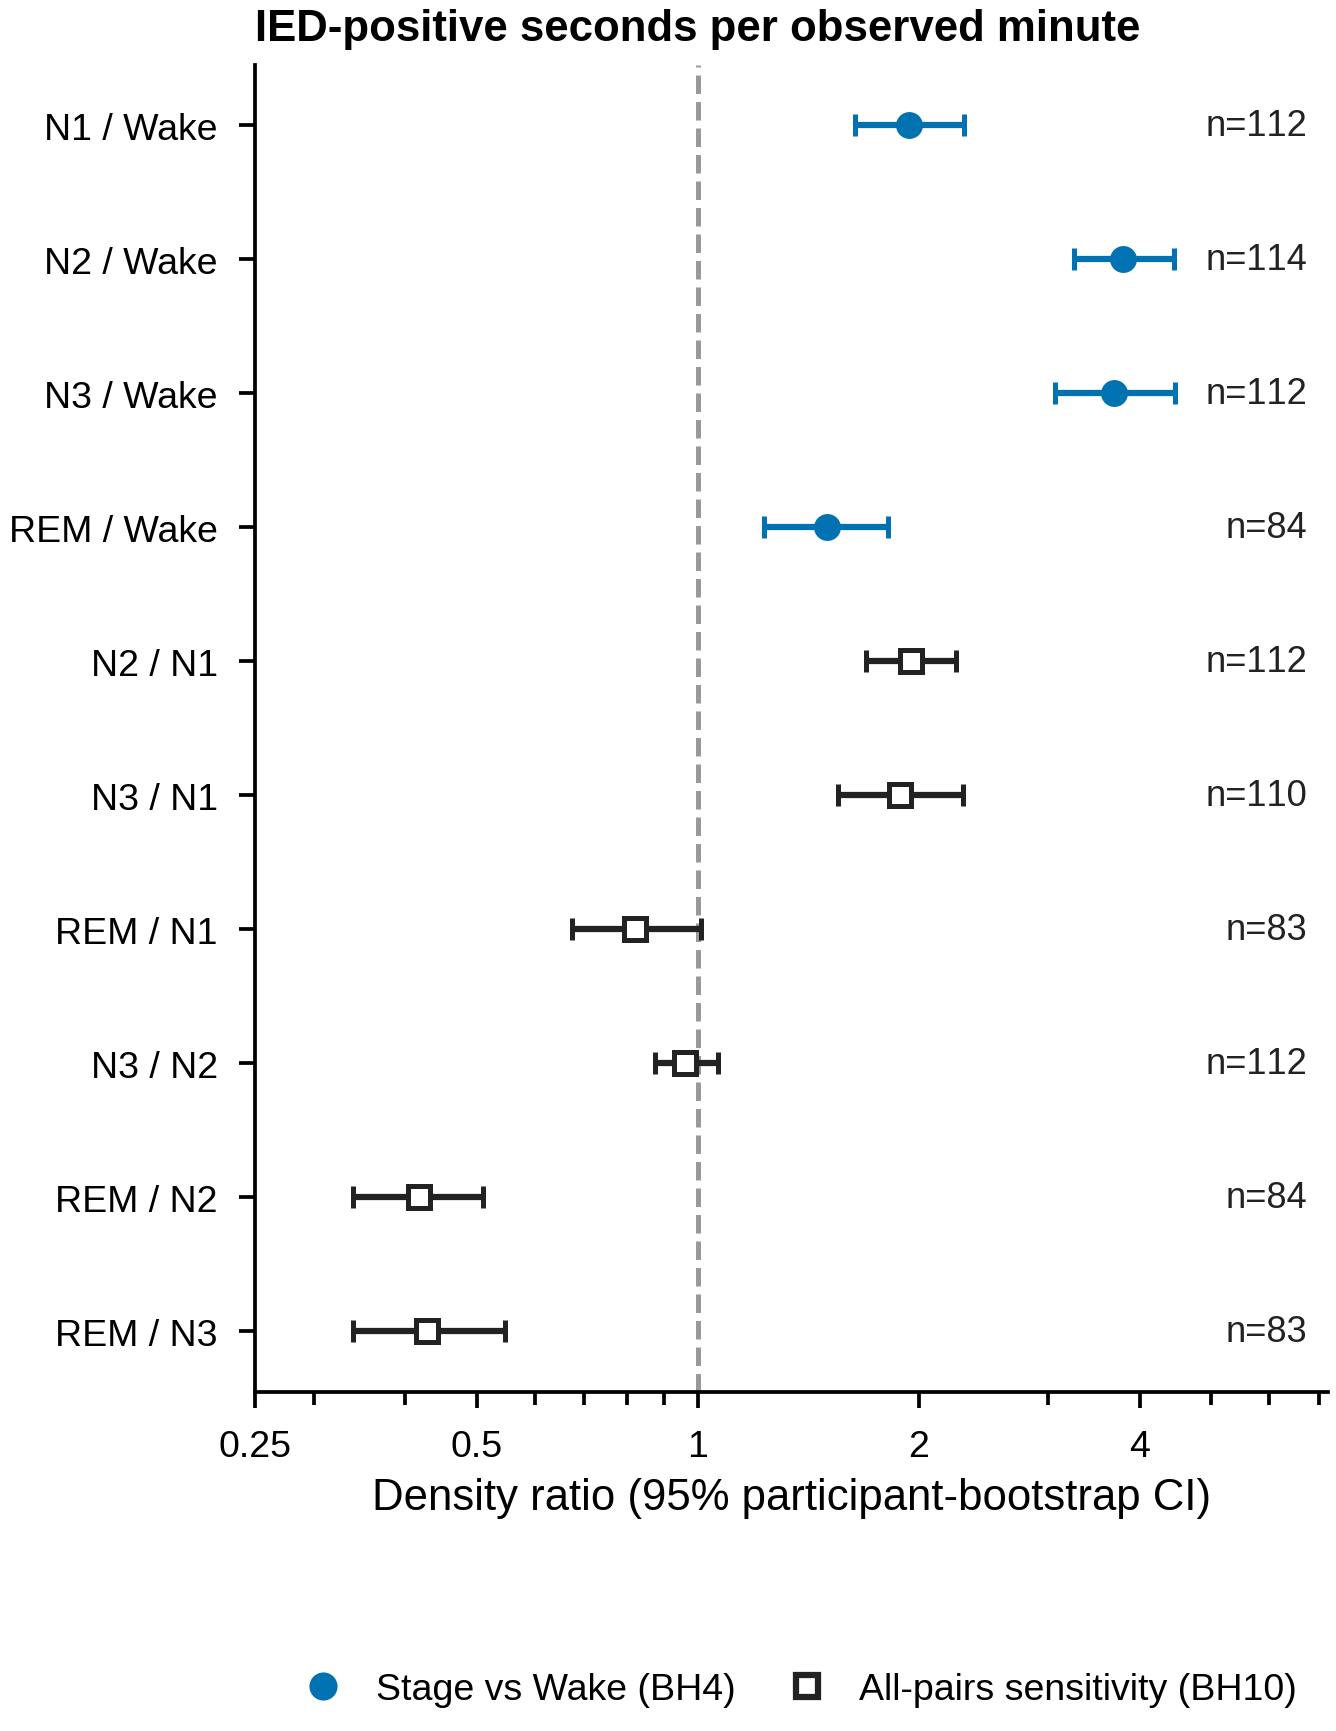
\includegraphics[width=0.52\textwidth]{figure_s1_sleep_contrasts.png}
\caption{Vigilance-state contrasts in IED-positive-second density. Points show geometric mean ratios and bars show percentile 95\% intervals from 5,000 patient-level bootstrap resamples. Stage/wake values were N1 1.94 (1.64--2.30; N1: n = 112), N2 3.80 (3.25--4.45; N2: n = 114), N3 3.69 (3.07--4.46; N3: n = 112), and REM 1.50 (1.23--1.82; REM: n = 84); all four stage-versus-wake signed-rank tests had $q<0.001$ after four-test Benjamini--Hochberg correction. N2 and N3 were each approximately 1.9-fold higher than N1; N2 and N3 did not differ ($q=0.38$). REM was 0.42-fold of N2 and 0.43-fold of N3 and was numerically lower than N1 ($q=0.051$). Blue circles denote the four primary stage-versus-wake contrasts; open squares denote contrasts from the separate all-ten-pair family. Correction applied to signed-rank tests, not plotted intervals.}
\label{fig:sleep-contrasts}
\end{figure}

\clearpage
\begin{figure}[H]
\centering
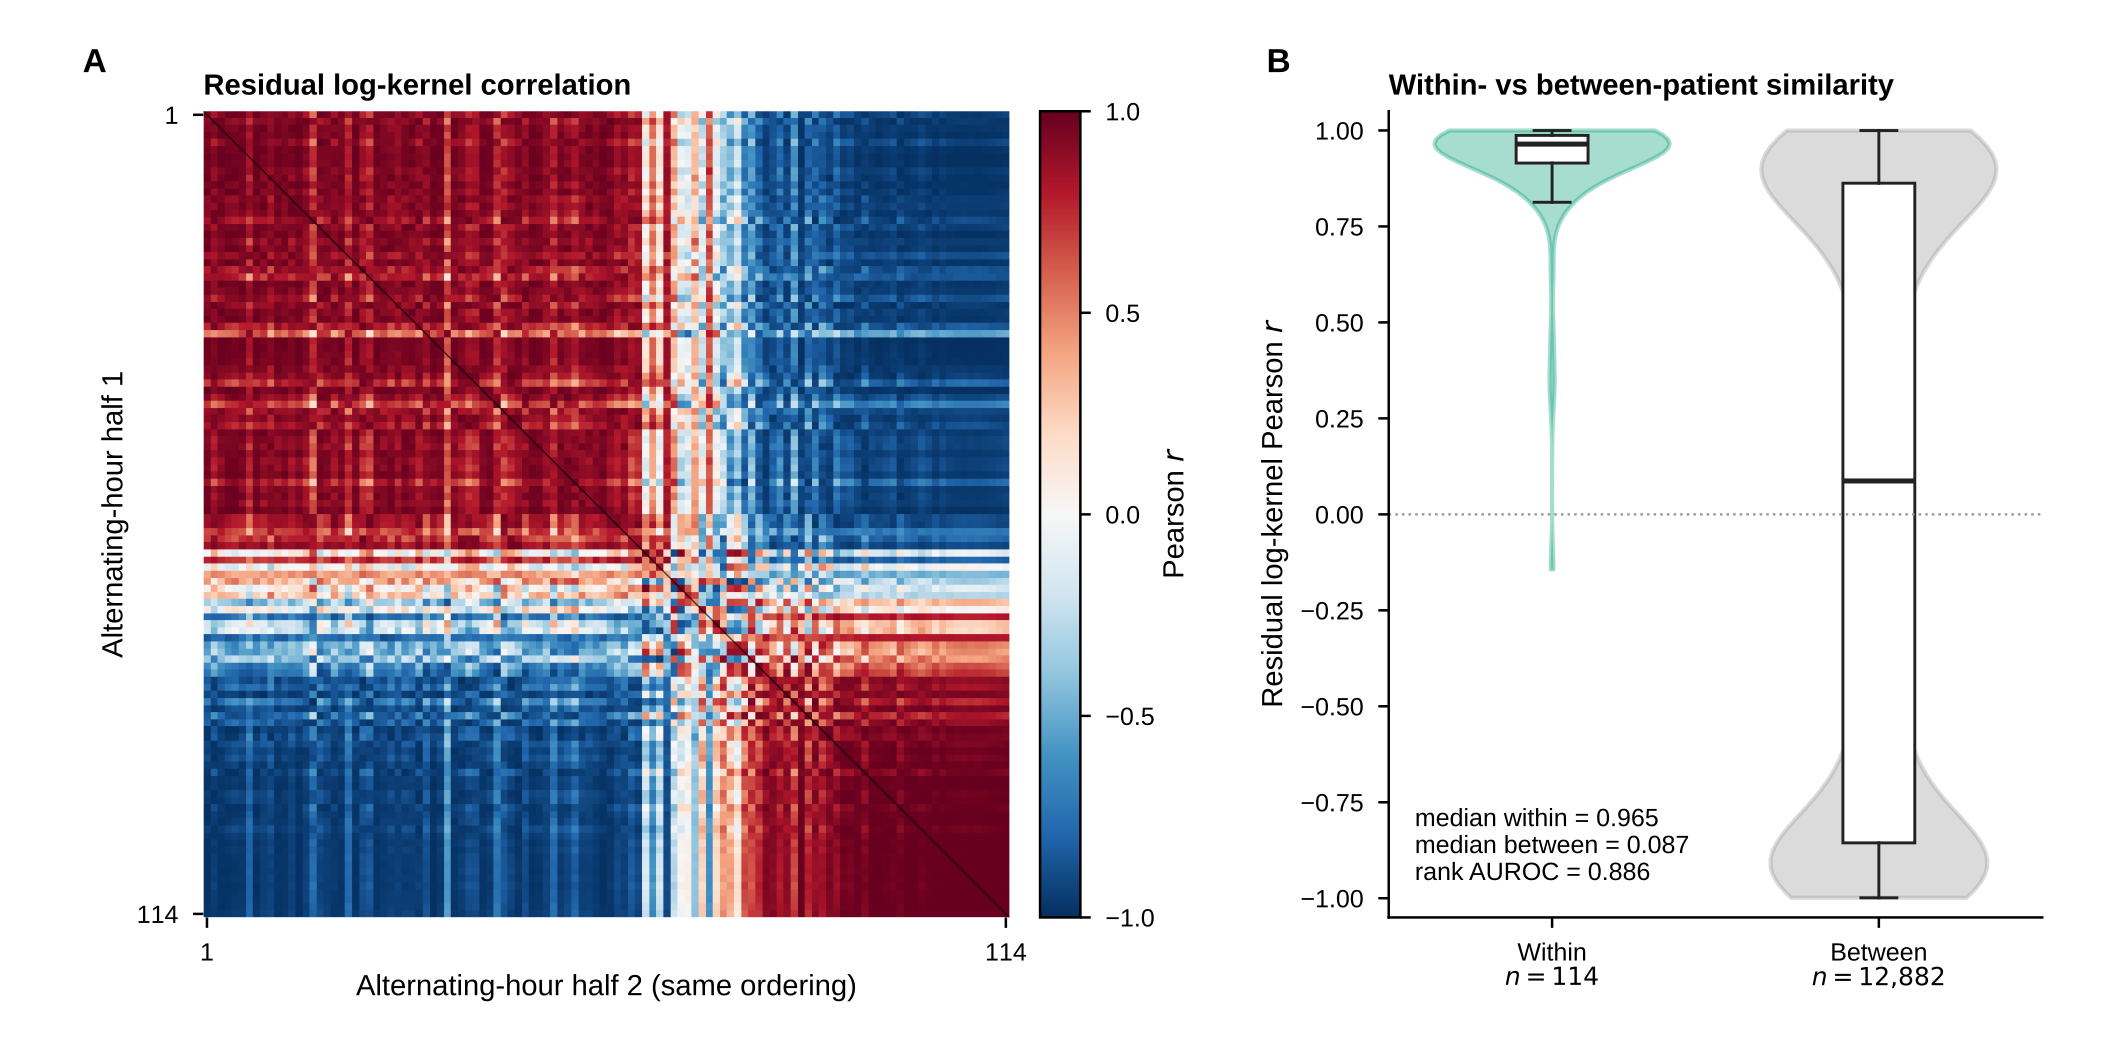
\includegraphics[width=\textwidth]{figure_s2_history_perturbation.png}
\caption{Within-admission split-half reproducibility of history kernels. \textbf{A}, Cross-half correlations between residualized 1--15-s log-kernel curves estimated independently from alternating-clock-hour portions for all 114 patients. Rows and columns share the same unsupervised ordering. \textbf{B}, Within-patient and directed between-patient correlations. Median correlation was 0.965 within patients (IQR 0.915--0.987) and 0.087 between patients across 12,882 pairs; AUROC was 0.886.}
\label{fig:history-perturbation-matrix}
\end{figure}

\clearpage
\begin{figure}[H]
\centering
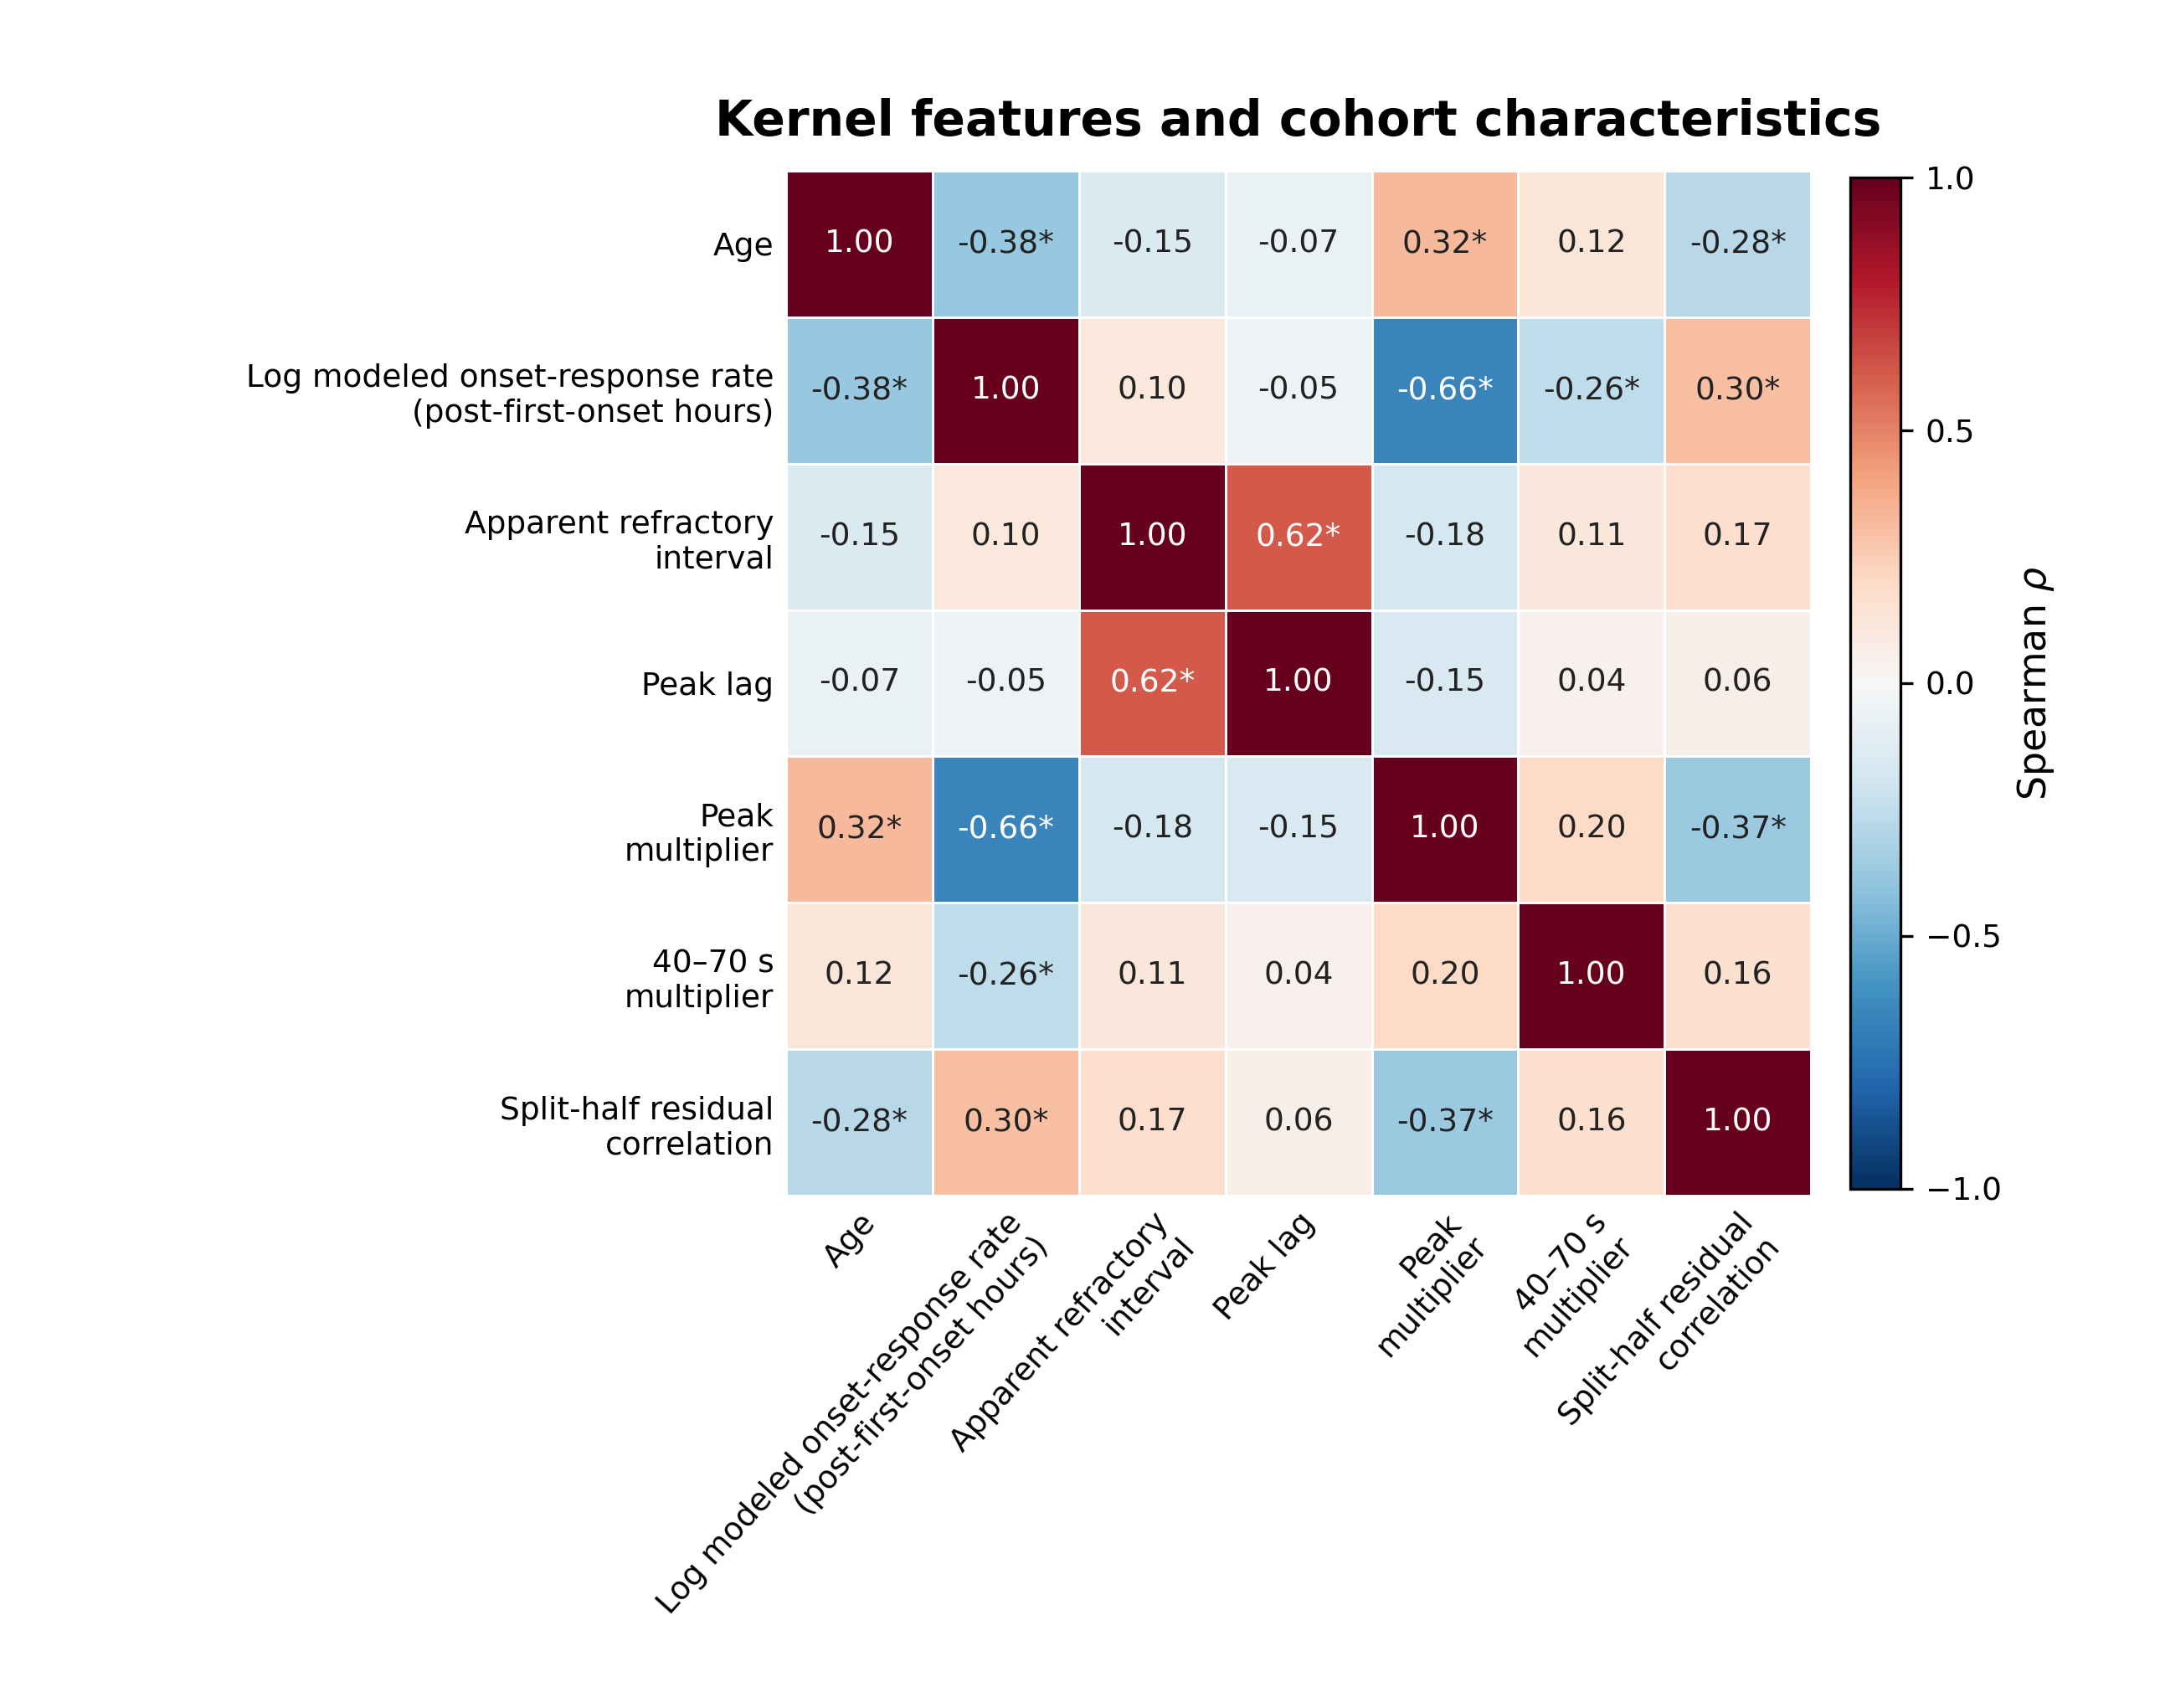
\includegraphics[width=0.76\textwidth]{figure_s3_kernel_correlations.png}
\caption{Relationships among cohort characteristics and history-kernel features. Cells show Spearman correlations across 114 patients; asterisks denote Benjamini--Hochberg-adjusted $q<0.05$ across 21 unique pairs. The modeled onset-response rate is the merged-onset response count divided by post-first-onset modeled hours (with the denominator rounded to 0.1 h) and is plotted on a logarithmic scale. The apparent refractory interval is constrained by the merged-onset procedure.}
\label{fig:kernel-feature-correlations}
\end{figure}

\clearpage
\begin{figure}[H]
\centering
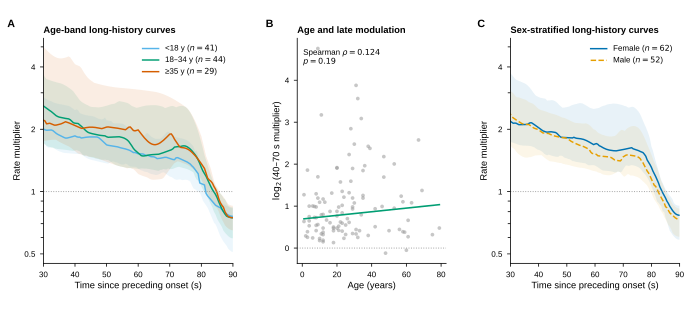
\includegraphics[width=\textwidth]{figure_s4_demographic_history.png}
\caption{Demographic variation in extended history kernels. \textbf{A}, Median 30--90-s multipliers and interquartile bands by age group. \textbf{B}, Age versus the $\log_2$ mean 40--70-s multiplier with Theil--Sen trend ($\rho=0.124$, $p=0.190$). \textbf{C}, Median curves and interquartile bands by sex. Group summaries are unadjusted and use patient-specific multiplier references.}
\label{fig:demographic-history}
\end{figure}

\clearpage
\addcontentsline{toc}{section}{SI References}
\renewcommand{\refname}{SI References}
\begin{thebibliography}{99}
\bibitem{MORGOTHValidation2026} Sun C, Karakis I, Herlopian A, et al. Toward unified and comprehensive automated EEG interpretation: multi-center development and validation of an EEG foundation model. \textit{Lancet Digit Health}. In press. 2026.
\bibitem{MORGOTH2026} Sun C, Karakis I, Herlopian A, et al. \textit{MORGOTH 1.0: A Foundation Model for Clinical EEG---Data and Code}. Version 1.0.0. Brain Data Science Platform; 2026. doi:10.60508/v7ky-5g40.
\bibitem{Jing2020} Jing J, Sun H, Kim JA, et al. Development of expert-level automated detection of epileptiform discharges during electroencephalogram interpretation. \textit{JAMA Neurol}. 2020;77:103--108.
\bibitem{Truccolo2005} Truccolo W, Eden UT, Fellows MR, Donoghue JP, Brown EN. A point process framework for relating neural spiking activity to spiking history, neural ensemble, and extrinsic covariate effects. \textit{J Neurophysiol}. 2005;93:1074--1089.
\bibitem{Paninski2004} Paninski L. Maximum likelihood estimation of cascade point-process neural encoding models. \textit{Network}. 2004;15:243--262.
\bibitem{Ghosn2023} Ghosn NJ, Xie K, Pattnaik AR, et al. A pharmacokinetic model of antiseizure medication load to guide care in the epilepsy monitoring unit. \textit{Epilepsia}. 2023;64:1236--1247. doi:10.1111/epi.17558.
\bibitem{GhosnSoftware} Ghosn NJ. \textit{ASM Project}. 2022. \url{https://github.com/nghosn3/ASM-project}.
\bibitem{Sarmashghi2021} Sarmashghi M, Jadhav SP, Eden UT. Efficient spline regression for neural spiking data. \textit{PLoS One}. 2021;16:e0258321.
\bibitem{Benjamini1995} Benjamini Y, Hochberg Y. Controlling the false discovery rate: a practical and powerful approach to multiple testing. \textit{J R Stat Soc Series B}. 1995;57:289--300.
\end{thebibliography}

\end{document}
